
\section{Angle dependent measurements}
    \label{Sec:3:AngleDependentMeasurements}

Preliminary measurements showed very strong dHvA oscillations which begin at relatively low field.  An example of the raw data can be seen in \fig~\ref{Fig:3:RawOscillations}. Since is is not clear from the raw torque data where the oscillations begin, Fourier transforms were taken over a small field range, for example \unit[1]{T} -- the interval where a clear signal is present marks the onset of oscillations. A FFT of the data between \unit[6]{T} and \unit[7]{T} is shown in the inset of the figure. This clearly shows the electron peaks at \unit[1370]{T}, \unit[2175]{T} and \unit[2343]{T}, whereas below \unit[6]{T} there was no appreciable signal. For subsequent measurements the field was ramped between \unit[6]{T} and the safe maximum of $\unit[18]{T}$ unless otherwise stated.
%%
\begin{figure}[h!]
    \begin{center}
        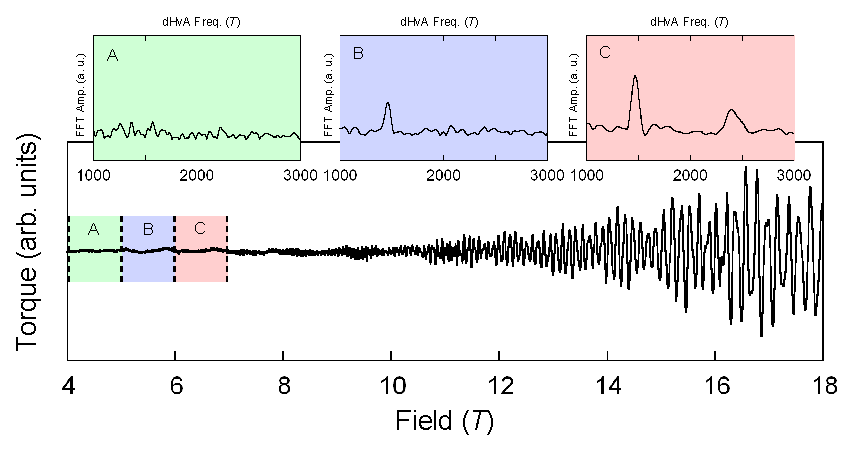
\includegraphics[scale=0.7]{Chapter3-dHvABaFe2P2/Figures/AngleDepMeasurements/RawOscillations/RawOscillations}
        \caption{An example of the torque data taken with field aligned at \unit[9]{\degree} from the $[001]$ direction. Inset shows a FFT of the data between \unit[6]{T} and \unit[8]{T}}
        \label{Fig:3:RawOscillations}
    \end{center}
\end{figure}


 \Fig~\ref{Fig:3:ComparisonSweepRates} shows some example Fourier transforms of data taken at various sweep rates. Since there is little difference between the sweeps at \unit[0.05]{T/min.} and \unit[0.1]{T/min.}, subsequent sweeps were performed at \unit[0.1]{T/min.}.
%%
\begin{figure}[h!]
    \begin{center}
        \includegraphics[scale=0.7]{Chapter3-dHvABaFe2P2/Figures/AngleDepMeasurements/SweepRateComparison/SweepRateComparison}
        \caption{FFTs showing the peak from the smaller branch of band $3$ shifted arbitrarily for comparison with the $H$ field at \unit[10]{\degree} from $[001]$ in the $[110]$ direction. Sweeps were performed at, A: \unit[0.05]{T/min.}, B: \unit[0.1]{T/min.} and C: \unit[0.2]{T/min.}}
        \label{Fig:3:ComparisonSweepRates}
    \end{center}
\end{figure}

Measurements were taken at one degree intervals from $H || [001]$ down to $H || [100]$ and from $H || [001]$ down to $H || [110]$. \Fig~\ref{Fig:3:FFTExamples} shows three example FFTs which show all the bands identified the next section. They also show first and second harmonics\footnote{Third harmonics were also identified in other FFTs, these are marked in \fig~\ref{Fig:3:AngleSweepMeasured}.}.
%%
\begin{figure}[h!]
    \begin{center}
        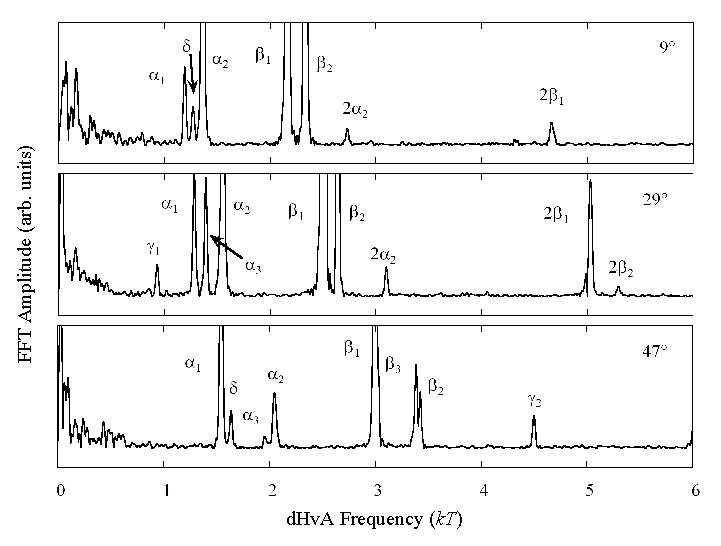
\includegraphics[scale=0.7]{Chapter3-dHvABaFe2P2/Figures/AngleDepMeasurements/FFTExamples/FFTExamples}
        \caption{FFT after a polynomial background was subtracted at various labeled angles. Peak identification is explained in the next section.}
        \label{Fig:3:FFTExamples}
    \end{center}
\end{figure}

The low frequency region in \fig~\ref{Fig:3:FFTExamples} shows noise from the cantilever, but according to DFT fits performed in the next section, this region also likely contains signal from the minimum of band $1$. Given that the signal from electron bands is generally small due to high scattering rate, we were not able to extract a convincing Fourier peak.

\Fig~\ref{Fig:3:AngleSweepMeasured} shows the set of peak data after having the angle determined as described in section~\ref{Sec:2:DeterminingAngle}. The Points marked in grey are the harmonics which were identified by overlaying the measured data on itself after doubling and tripling of the frequency.
%%
\begin{figure}[h!]
    \begin{center}
        \includegraphics[scale=0.7]{Chapter3-dHvABaFe2P2/Figures/AngleDepMeasurements/AngleSweepMeasured/AngleSweepMeasured}
        \caption{Peaks identified by varying the field range, window type and background polynomial. Left panel shows data taken with the field parrallel to $[001]$ down to $[110]$, the right panels shows $[001]$ to $[100]$. Points marked in grey are harmonics.}
        \label{Fig:3:AngleSweepMeasured}
    \end{center}
\end{figure}

    \begin{center}
        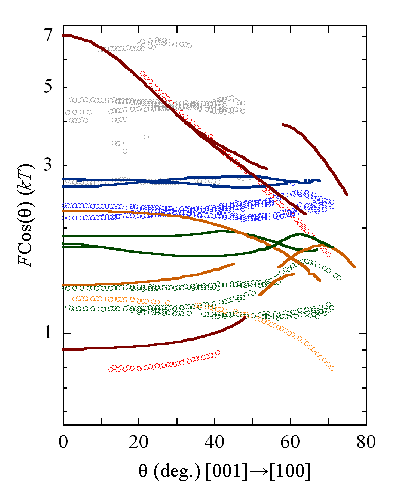
\includegraphics[scale=0.7]{Chapter3-dHvABaFe2P2/Figures/AngleDepMeasurements/AngleSweepMeasuredUnshifted/AngleSweepMeasuredUnshifted}
        \caption{dHvA frequencies multipled by $\cos(\theta)$. Solid lines are DFT calculations, open circles are measured data. $H$ field directed along $[001]\rightarrow[100]$.}
        \label{Fig:3:AngleSweepUnshifted}
    \end{center}
\end{figure}

For the $[110]$ direction it became apparent from the fact that the DFT and the measured curves were qualitatively different that the field was not perfectly aligned with the $[110]$ axis of the sample. By assuming that the measurements were taken from the $c$-axis direction down to a vector rotated \unit[10]{\degree} within the $ab$-plane from the $[110]$ direction, the DFT data matches much better. This is within the estimated error for alignment from the microscope images.


\subsubsection{Rigidly shifting the calculated DFT energies}

As is shown in \fig~\ref{Fig:3:ComparisonRotationPlotUnshiftedDFT}, the rotation plots from the DFT calculations match up qualitatively with the data but do not match up quantitatively -- the electron bands overestimating the size of the measured extremal orbits by around TODO and the hole orbits overestimating the extremal orbits by around TODO. 

\begin{figure}[h!]
    \begin{center}
        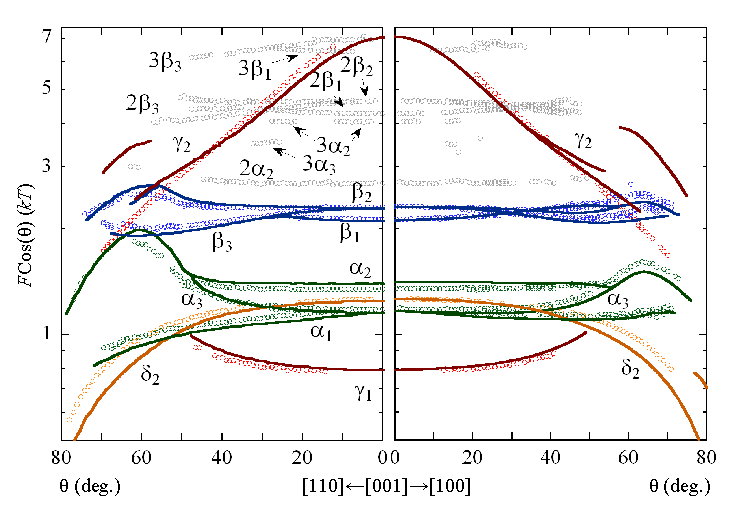
\includegraphics[scale=0.7]{Chapter3-dHvABaFe2P2/Figures/AngleDepMeasurements/AngleSweepRigidShift/AngleSweepRigidShift}
        \caption{dHvA frequencies multipled by $\cos(\theta)$. Solid lines are rigidly shifted DFT calculations, open circles are measured data. $H$ field directed along $[001]$ towards (a) $[001]\rightarrow[100]$ and (b) $[001]\rightarrow[110]$.}
        \label{Fig:3:AngleSweepRigidShift}
    \end{center}
\end{figure}

In order to obtain the correct shape of Fermi surface, the DFT calculations need to be tweaked. One technique is to apply small band-specific rigid energy shifts, which, in most cases is enough to bring the DFT in line with the experimental data. \fig~\ref{Fig:3:AngleSweepRigidShift} shows the rotation plots which rotate towards both the 100 and 110 directions along with appropriately shifted calculations. Table~\ref{Table:3:EnergyShifts} lists those energy shifts.

\medskip

\begin{center}
    \begin{tabular}[h!]{llr}
\toprule
Band    & \multicolumn{2}{l}{Energy Shift (\unit{Ry})} \\
\midrule
1       &       & -0.0083      \\
2       & Wide  & 0.0          \\
        & Narrow & -0.0038     \\
3       &       & 0.0043       \\
4       &       & 0.0050        \\
\bottomrule
    \label{Table:3:EnergyShifts}
    \end{tabular}
\end{center}

Band $2$ in this case has two separate shifts specified in two different regions of the Brillouin zone. The rotation plot for the wider orbit located at the edge of the Brillouin zone was calculated with no energy shift and the narrow part of the Fermi surface around the $\Gamma$ point was calculated with a shift of $0.0038\unit{Ry}$. This provides a reasonable match for the rotation plot where we can apply the shift to the two regions discretely, however is proves problematic when we wish to study intermediate areas since it is not clear how the Fermi surface varies between the two regions.

\subsubsection{Shifting the DFT calculations proptional to orbital character}
\label{Sec:ShiftingDFTPropToOrbitalCharacter}

\Fig~\ref{Fig:3:Band2DCharacter} shows the strength of various d-orbital band characters taken on a 110 cut through the \BaFeP Brillouin zone with the band $2$ Fermi surface superimposed. Band characters for the other bands can be found in Appendix~\ref{TODO}.
%%
\begin{figure}[h!]
    \begin{center}
        \includegraphics[scale=0.7]{Chapter3-dHvABaFe2P2/Figures/AngleDepMeasurements/BandCharacterPlot/Band2_110Slice_BandCharacter}
        \caption{Partial $d$-orbital character of the hole band $2$ across slices in the 110 direction. Solid lines show the Fermi surface in the plane.}
        \label{Fig:3:Band2DCharacter}
    \end{center}
\end{figure}
%%
\begin{figure}[h!]
    \begin{center}
        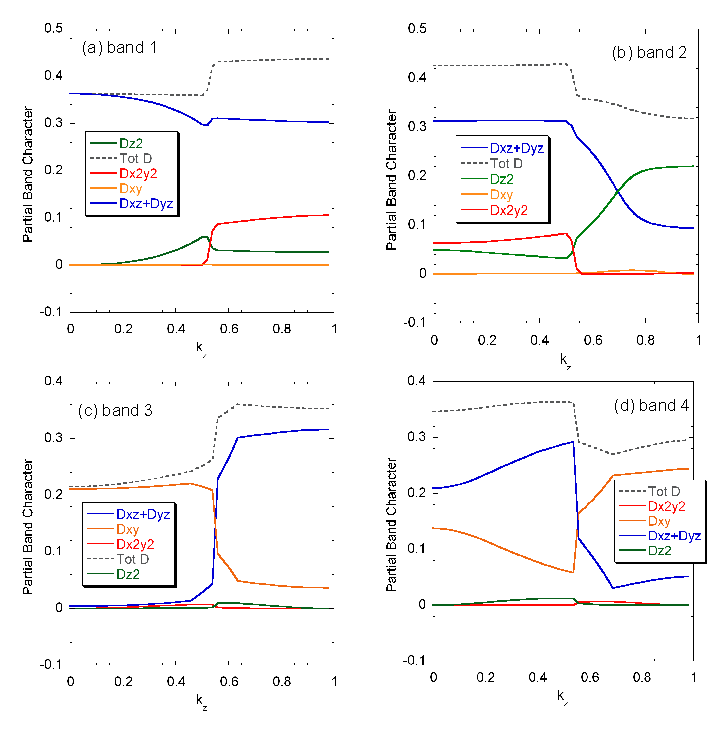
\includegraphics[scale=0.7]{Chapter3-dHvABaFe2P2/Figures/AngleDepMeasurements/BandCharacterVsKz/BandCharacterVsKz}
        \caption{Partial $d$-orbital characters of the hole band $2$ along the Fermi surface in the 110 slice vs. \kz}
        \label{Fig:3:Band2DCharacterVsKz}
    \end{center}
\end{figure}

Band $2$ has very little \Dxy and \DxTwoyTwo character close to the Fermi level but shows a significant amount of \DzTwo character at the wide region of the Fermi surface and \DxzDyz character at the narrow region. \Fig~\ref{Fig:3:Band2DCharacterVsKz} shows the orbital character for each of the $d$-orbitals as a function of \kz along the Fermi surface. Evidently, energy shifts could be applied which are scaled to either the \DzTwo and \DxzDyz orbital character in order that we obtain a smooth energy shift transition between the narrow and wide regions discussed previously.

Energy shifts were applied across the full $3$d Brillouin zone for band $2$ using the following two scalings,
%%
\begin{align*}
\textrm{\DzTwo:}\quad \Delta\epsilon &= 0.002 - 0.0052 (1 - (\epsilon - 0.033)/(0.2205 - 0.033)) \\
\textrm{\DxzDyz:}\quad \Delta\epsilon &= 0.002 - 0.0052 (\epsilon - 0.0946)/(0.3135 - 0.0946)
\end{align*}
%%
Note that these scalings ensure that the energy shift applied varies between $-0.0032\unit{Ry}$ and $0.002\unit{Ry}$ which are slightly different to the values applied when rigidly shifting the band. This is due to the fact that the Fermi surface area measured in one region is affected more and more by the size of the Fermi surface in the opposite region as the azimuthal angle gets higher and the calculated area deviates from the measured area. This is what results in the crossing of the calculated rotation plot with the measured rotation plot shown in the first panel of \fig~\ref{Fig:3:Band2DCharacterRigidComparison}. A rigid shift was therefore chosen which best lines up along the length of the curve -- one which will be slightly lower than if we were to match the plots exactly at the 001 direction.

\begin{figure}[h!]
    \begin{center}
        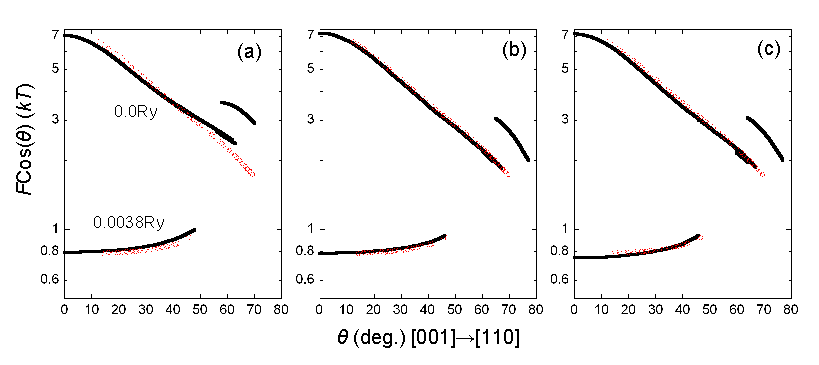
\includegraphics[scale=0.7]{Chapter3-dHvABaFe2P2/Figures/AngleDepMeasurements/BandCharacterRotPlot/Band2_110_RotPlot_Comparison}
        \caption{dHvA frequencies for band 2 multipled by the cosine of the angle of the $H$ field. $H$ field directed along $[001]\rightarrow[110]$. Open circles are measured data, solid lines represent (a) rigidly shifted DFT calculations, (b) DFT calculations shifted proportional to \DzTwo orbital character, (c) DFT calculations shifted proportional to \DxzDyz orbital character.}
        \label{Fig:3:Band2DCharacterRigidComparison}
    \end{center}
\end{figure}

The second and third panels of \fig~\ref{Fig:3:Band2DCharacterRigidComparison} show the rotation plots calculated with the energy shifts applied proportional to \DzTwo and \DxzDyz orbital character respecitvely. We observe a much better alignment of the measured and calculated data for all angles. \Fig~\ref{Fig:3:BandCharacterFSShiftComparison} shows the Fermi surfaces before and after shifting using the rigid energy shifts for bands $1$, $3$ and $4$ and using shifts scaled to \DzTwo orbital character for band $2$, as well as incorporating the corrections discussed in section~\ref{Sec:3:MappingFermiSurfaceDFTCalulations}. \Fig~\ref{Fig:3:FullBandCharacterFermiSurface} shows the assembled unit cell for \BaFeP from the corrected DFT calculations.
%%
\begin{figure}[h!]
    \begin{center}
        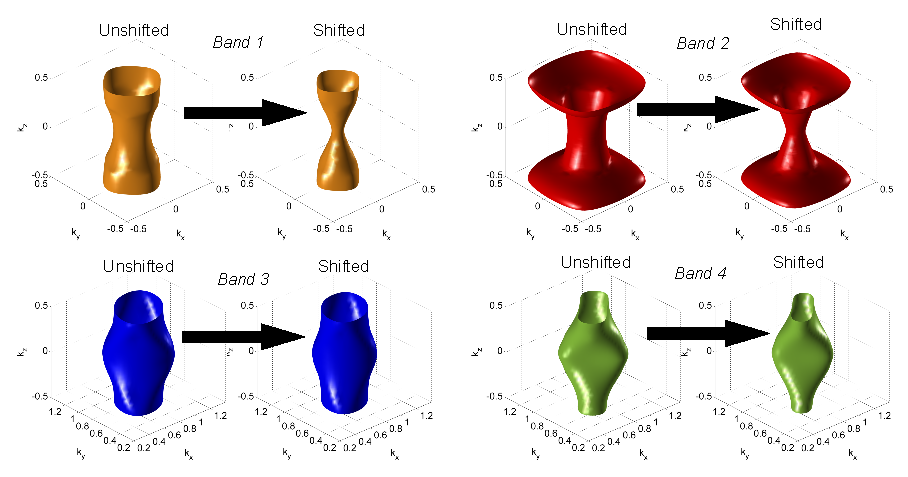
\includegraphics[scale=0.7]{Chapter3-dHvABaFe2P2/Figures/AngleDepMeasurements/BandCharacterFermiSurface/BandCharacterFermiSurfaceShiftComparison}
        \caption{Comparison of Fermi surfaces according to DFT calculations both before and after shift corrections are applied. Rigid shifts are applied to bands 1, 3, 4 and shifts proprtional to \DzTwo character are applied to band 2.}
        \label{Fig:3:BandCharacterFSShiftComparison}
    \end{center}
\end{figure}
%%
\begin{figure}[h!]
    \begin{center}
        \includegraphics[scale=0.7]{Chapter3-dHvABaFe2P2/Figures/AngleDepMeasurements/BandCharacterFermiSurface/FullBandCharacterFermiSurface}
        \caption{Fully assembled Fermi surface in the first Brillouin of \BaFeP as determined by DFT calculations corrected by either rigid energy shifts (bands 1, 3, 4) or shifts proprtional to \DzTwo character (band 2)}
        \label{Fig:3:FullBandCharacterFermiSurface}
    \end{center}
\end{figure}


\subsection{Tight binding model fits}


\subsection{Susceptibility calculations}
\label{Sec:SubsceptibilityCalculation}



